% !TeX program = lualatex
\documentclass[11pt,a4paper]{article}
\usepackage{szzmaterial}
\setlist[enumerate]{nosep,leftmargin=2.1em}
\setlist[itemize]{nosep,leftmargin=1.8em}

\szztitul{Základy diferenciálního a integrálního počtu}{M1}{NMAI054 (Matematická analýza 1)}

\newcommand{\playlist}{https://www.youtube.com/playlist?list=PLZHQObOWTQDMsr9K-rj53DwVRMYO3t5Yr}

\begin{document}
\maketitle
\tableofcontents
\bigskip

\section*{Úvod}
\addcontentsline{toc}{section}{Úvod}

Tento materiál pokrývá okruh \textbf{M1 -- Základy diferenciálního a integrálního počtu} (předmět NMAI054, Matematická analýza~1). Výklad je postaven primárně na zápiscích z přednášky doc.~Jelínka; značení a hloubka odpovídají kurzu pro informatiky.

Věty uvádíme \emph{se zněním}, doplněné intuicí a krátkými odvozeními tam, kde pomáhají pochopení; rozsáhlé formální důkazy vynecháváme. Do výkladu jsou zařazeny řešené reálné otázky SZZ z let 2022--2026; všechny otázky k okruhu jsou pohromadě v samostatném dokumentu \emph{Příklady otázek}. Použité zdroje jsou uvedeny na konci.

\medskip
\noindent\textbf{Značení.} $\mathbb{N}=\{1,2,\dots\}$, $\mathbb{R}$ jsou reálná čísla a $\mathbb{R}^*=\mathbb{R}\cup\{-\infty,+\infty\}$ je množina \emph{rozšířených} reálných čísel. \emph{Okolím} bodu $a\in\mathbb{R}$ rozumíme interval $U(a,\delta)=(a-\delta,a+\delta)$, \emph{prstencové okolí} $P(a,\delta)=U(a,\delta)\setminus\{a\}$ je okolí bez bodu~$a$. Okolí nekonečen: $U(+\infty,\delta)=(1/\delta,+\infty)$, $U(-\infty,\delta)=(-\infty,-1/\delta)$.

% ============================================================
\section{Posloupnosti reálných čísel a jejich limity}

Posloupnost je zobrazení $\mathbb{N}\to\mathbb{R}$, píšeme $(a_n)_{n=1}^\infty$. Základní otázkou je, zda se členy posloupnosti k něčemu \uv{blíží}, a pokud ano, k čemu. To formalizuje pojem limity.

\begin{definice}[Limita posloupnosti]
Řekneme, že posloupnost $(a_n)$ má \emph{limitu} $a\in\mathbb{R}^*$, píšeme $\lim_{n\to\infty}a_n=a$, pokud pro každé okolí $U(a,\varepsilon)$ existuje index $n_0$ tak, že $a_n\in U(a,\varepsilon)$ pro všechna $n>n_0$. Pro vlastní limitu $a\in\mathbb{R}$ to znamená
\[
  \forall\varepsilon>0\ \exists n_0\ \forall n>n_0:\ |a_n-a|<\varepsilon.
\]
Posloupnost s \emph{vlastní} limitou ($a\in\mathbb{R}$) se nazývá \emph{konvergentní}, jinak \emph{divergentní} (sem patří i nevlastní limity $\pm\infty$).
\end{definice}

\begin{intuice}
Od jistého indexu dál leží \emph{všechny} členy posloupnosti v libovolně malém okolí limity. \uv{Libovolně malé} se formalizuje jako \uv{pro každé $\varepsilon>0$}: čím menší $\varepsilon$ zvolíme, tím dál (větší $n_0$) možná musíme jít, ale vždy se to podaří.
\end{intuice}

\begin{definice}[Omezenost a monotonie]
Posloupnost $(a_n)$ je \emph{shora omezená}, existuje-li $K\in\mathbb{R}$ s~$a_n\le K$ pro všechna $n$; \emph{zdola omezená} obdobně ($a_n\ge K$); \emph{omezená}, je-li omezená shora i~zdola. Dále je $(a_n)$ \emph{neklesající}, platí-li $a_n\le a_{n+1}$ pro všechna $n$, \emph{nerostoucí} při $a_n\ge a_{n+1}$, \emph{rostoucí} při $a_n<a_{n+1}$ a~\emph{klesající} při $a_n>a_{n+1}$. Je \emph{monotónní}, je-li neklesající nebo nerostoucí (\emph{ryze monotónní} při rostoucí či klesající). Pro funkci $f$ na intervalu $J$ se tytéž pojmy zavádějí přes funkční hodnoty: např.\ $f$ je \emph{rostoucí}, platí-li $f(x)<f(y)$ pro každá $x<y$ z~$J$ (ostatní varianty obdobně).
\end{definice}

Limita je určena jednoznačně. Dále platí, že každá konvergentní posloupnost je omezená (opak neplatí: $a_n=(-1)^n$ je omezená, ale nemá limitu). Důležitou postačující podmínkou pro existenci limity je monotonie:

\begin{veta}[Limita monotónní posloupnosti]
Každá monotónní posloupnost má limitu (případně nevlastní). Je-li navíc omezená, je tato limita vlastní, takže posloupnost konverguje.
\end{veta}

Pro praktický výpočet limit slouží aritmetika limit. Pozor: funguje jen tehdy, je-li pravá strana definovaná (neurčité výrazy jako $\infty-\infty$, $0\cdot\infty$, $\infty/\infty$, $a/0$ jsou vyloučené).

\begin{veta}[Aritmetika limit]
Nechť $\lim a_n=a\in\mathbb{R}^*$ a $\lim b_n=b\in\mathbb{R}^*$. Pak (pokud je pravá strana definována)
\[
  \lim(a_n+b_n)=a+b,\quad \lim(a_n b_n)=a b,\quad \lim\frac{a_n}{b_n}=\frac{a}{b}\ (b_n\neq0).
\]
Navíc: je-li $(a_n)$ omezená a $\lim b_n=0$, pak $\lim(a_n b_n)=0$.
\end{veta}

\begin{poznamka}
Aritmetika limit je \emph{jednosměrná}. Z konvergence součtu $(a_n+b_n)$ neplyne konvergence jednotlivých posloupností: pro $a_n=(-1)^n$ a $b_n=-(-1)^n$ součet konverguje (k~0), ale ani jedna z posloupností limitu nemá.
\end{poznamka}

\begin{veta}[O limitě a uspořádání]
Nechť $\lim a_n=a$ a $\lim b_n=b$ (v $\mathbb{R}^*$). Pak
\begin{enumerate}
  \item je-li $a<b$, existuje $n_0$ tak, že $a_n<b_n$ pro všechna $n>n_0$;
  \item je-li $a_n\le b_n$ pro všechna $n>n_0$, pak $a\le b$.
\end{enumerate}
\end{veta}

\begin{poznamka}
Ostrá nerovnost se v limitě může \uv{zkazit} na neostrou: $a_n=1-\tfrac1n<1=b_n$ pro všechna $n$, ale obě limity jsou rovny~$1$.
\end{poznamka}

\begin{veta}[O dvou policajtech]
Nechť $\lim a_n=\lim b_n=a\in\mathbb{R}$ a pro všechna $n>n_0$ platí $a_n\le c_n\le b_n$. Potom $(c_n)$ konverguje a $\lim c_n=a$.
\end{veta}

\begin{intuice}
Posloupnost $(c_n)$ je \uv{sevřena} mezi dvěma posloupnostmi (\uv{policajty}), které míří do téhož bodu; nemá tedy kam jinam jít. Pro nevlastní limitu stačí jeden policajt: dolní odhad jdoucí do $+\infty$ vynutí $\lim c_n=+\infty$.
\end{intuice}

\begin{center}
\begin{tikzpicture}[x=1.0cm,y=2.1cm,>=stealth]
  \draw[->,gray!60](-0.2,0)--(7.4,0) node[right]{$x$};
  \draw[->,gray!60](0,-1.05)--(0,1.35) node[above]{$y$};
  % horni policajt b(x)=1/x
  \draw[red!70!black,thick,domain=0.78:7,smooth,samples=80] plot(\x,{1/\x});
  % dolni policajt a(x)=-1/x
  \draw[red!70!black,thick,domain=0.78:7,smooth,samples=80] plot(\x,{-1/\x});
  % sevrena c(x)=sin x / x
  \draw[blue!60!black,very thick,domain=0.45:7,smooth,samples=120] plot(\x,{sin(deg(\x))/\x});
  \node[red!70!black] at (6.0,0.34){\small $b(x)=\tfrac1x$};
  \node[red!70!black] at (6.0,-0.34){\small $a(x)=-\tfrac1x$};
  \node[blue!60!black] at (3.05,0.62){\small $c(x)=\tfrac{\sin x}{x}$};
\end{tikzpicture}\obrpopis{%
Funkce {\color{blue!60!black}$c(x)=\tfrac{\sin x}{x}$} je pro $x>0$ \uv{uvězněna} mezi {\color{red!70!black}$a(x)=-\tfrac1x$ a $b(x)=\tfrac1x$}. Oba policajti mají pro $x\to\infty$ limitu~$0$, proto ji má i~sevřená funkce.}
\end{center}

\begin{priklad}[Výpočet limity sevřením]
\textbf{Zadání.} Spočítejte $\lim_{n\to\infty}\dfrac{\sin n}{n}$.\par
\textbf{Řešení.} Protože $-1\le\sin n\le 1$, platí $-\tfrac1n\le\tfrac{\sin n}{n}\le\tfrac1n$. Krajní posloupnosti mají limitu~$0$, podle věty o dvou policajtech je tedy i $\lim\tfrac{\sin n}{n}=0$. (Alternativně: $\tfrac1n$ je nulová a $\sin n$ omezená, takže součin jde k~0.)
\end{priklad}

\begin{priklad}[SZZ podzim 2022 č.~3: Posloupnosti -- limita a omezenost] \szzotazka{podzim 2022}{3}{Posloupnosti (limita, omezenost)}\par
\textbf{Zadání.} Nechť $(a_n)$ je posloupnost reálných čísel. (1)~Definujte, co znamená, že $(a_n)$ je \emph{konvergentní} (má vlastní limitu). (2)~Definujte, co znamená, že $(a_n)$ je \emph{neomezená}. (3)~Dokažte, že je-li $(a_n)$ neomezená, pak nekonverguje.\par
\textbf{Řešení.}
\begin{enumerate}
  \item $(a_n)$ konverguje (má vlastní limitu $L\in\mathbb{R}$) právě tehdy, když $\forall\varepsilon>0\ \exists n_0\ \forall n\ge n_0:\ |a_n-L|<\varepsilon$.
  \item $(a_n)$ je \emph{omezená}, existuje-li $K>0$ s~$|a_n|\le K$ pro všechna~$n$; \emph{neomezená} znamená, že omezená není, tj.\ $\forall K>0\ \exists n:\ |a_n|>K$.
  \item Dokážeme obměnou: ukážeme, že každá konvergentní posloupnost je omezená. Nechť $a_n\to L$. Pro $\varepsilon=1$ existuje $n_0$ tak, že pro $n\ge n_0$ je $|a_n|\le|a_n-L|+|L|<|L|+1$. Mimo to zbývá jen konečně mnoho členů, takže s~$K=\max\{|a_1|,\dots,|a_{n_0-1}|,\,|L|+1\}$ platí $|a_n|\le K$ pro všechna~$n$. Je-li tedy $(a_n)$ neomezená, nemůže konvergovat.
\end{enumerate}
\end{priklad}

% ============================================================
\section{Řady}

Řada je formální nekonečný součet členů posloupnosti. Místo abychom sčítali \uv{všechno najednou}, sledujeme posloupnost částečných součtů a ptáme se na její limitu; tím se otázka o nekonečném součtu převede na limitu posloupnosti.

\begin{definice}[Řada, částečný součet, součet]
Nechť $(a_n)_{n\ge0}$ je posloupnost reálných čísel. \emph{$N$-tý částečný součet} řady $\sum_{n=0}^{\infty}a_n$ je $s_N=\sum_{n=0}^{N}a_n$. Pokud existuje vlastní limita $\lim_{N\to\infty}s_N$, řada \emph{konverguje} a tuto limitu nazýváme jejím \emph{součtem}. Jinak (limita neexistuje nebo je nevlastní) řada \emph{diverguje}.
\end{definice}

Nejdůležitějším příkladem je řada, jejíž členy tvoří geometrickou posloupnost.

\begin{definice}[Geometrická řada]
Řada $\sum_{n=0}^{\infty}a_n$ je \emph{geometrická}, právě když $a_n=q^n$ pro nějaké $q\in\mathbb{R}$; číslu $q$ říkáme \emph{kvocient}.
\end{definice}

U geometrické řady umíme součet spočítat přesně. Pro $q\neq1$ má částečný součet uzavřený tvar $s_N=1+q+\dots+q^N=\dfrac{q^{N+1}-1}{q-1}$ (ověří se vynásobením $(q-1)s_N$). O chování součtu pak rozhoduje jen to, co dělá mocnina $q^{N+1}$:

\begin{veta}[Součet geometrické řady]
\[
  \sum_{n=0}^{\infty}q^n=
  \begin{cases}
    \dfrac{1}{1-q} & \text{pro } |q|<1,\\[2mm]
    +\infty & \text{pro } q\ge1,\\[1mm]
    \text{neexistuje} & \text{pro } q\le-1.
  \end{cases}
\]
\end{veta}

\begin{intuice}
Pro $|q|<1$ se členy $q^n$ zmenšují geometricky rychle, takže nekonečný součet \uv{doběhne} ke konečné hodnotě (z $q^{N+1}\to0$ plyne $s_N\to\tfrac{0-1}{q-1}=\tfrac1{1-q}$). Pro $q\ge1$ se členy nezmenšují a součet roste do $+\infty$; pro $q\le-1$ hodnota $q^{N+1}$ střídá znaménko a v absolutní hodnotě neklesá, takže limita neexistuje.
\end{intuice}

\begin{poznamka}
\uv{Členy jdou k nule} je pro konvergenci nutné, ale \emph{nestačí}. Učebnicový protipříklad je \emph{harmonická řada} $\sum_{n\ge1}\tfrac1n$: členy klesají k nule, ale řada diverguje. Obecněji $\sum_{n\ge1}\tfrac1{n^s}$ konverguje právě pro $s>1$ (důkaz integrálním kritériem, viz sekci o~integrálech).
\end{poznamka}

\video{https://www.youtube.com/watch?v=WUvTyaaNkzM}{3Blue1Brown, \emph{Essence of Calculus} kap.~1 -- \emph{The essence of calculus} (vizuální intuice k~nekonečným součtům a~kalkulu).}

\begin{priklad}[SZZ podzim 2023 č.~4: Geometrická řada] \szzotazka{podzim 2023}{4}{Geometrická řada}\par
\textbf{Zadání.} Sečtěte $\dfrac{4}{9}+\dfrac{8}{27}+\dfrac{16}{81}+\cdots$.\par
\textbf{Řešení.} Členy jsou tvaru $\left(\tfrac23\right)^2\left(\tfrac23\right)^n$, jde tedy o geometrickou řadu s kvocientem $q=\tfrac23$. Po vytknutí $(2/3)^2$ a dosazení do vzorce:
\[
  \left(\tfrac23\right)^2\sum_{n\ge0}\left(\tfrac23\right)^n=\frac{(2/3)^2}{1-2/3}=\frac{4}{3}.
\]
\end{priklad}

% ============================================================
\section{Reálné funkce jedné proměnné: limity a spojitost}

Pojem limity přenášíme z posloupností na funkce. Funkce $f$ je definovaná na nějaké podmnožině $\mathbb{R}$; limitu v bodě zkoumáme na prstencovém okolí (hodnota v samotném bodě limitu neovlivní).

\subsection{Limita funkce v bodě}

\begin{definice}[Limita funkce]
Funkce $f$ má v bodě $a\in\mathbb{R}^*$ \emph{limitu} $A\in\mathbb{R}^*$, píšeme $\lim_{x\to a}f(x)=A$, pokud
\[
  \forall\varepsilon>0\ \exists\delta>0:\ x\in P(a,\delta)\ \Rightarrow\ f(x)\in U(A,\varepsilon).
\]
\emph{Jednostranné} limity $\lim_{x\to a^+}f$, resp. $\lim_{x\to a^-}f$, definujeme nahrazením $P(a,\delta)$ pravým, resp. levým prstencovým okolím. Platí: $\lim_{x\to a}f=A$ právě tehdy, když obě jednostranné limity existují a rovnají se $A$.
\end{definice}

\begin{intuice}
Blíží-li se $x$ k~$a$ (zleva i zprava, ale $x\neq a$), blíží se $f(x)$ k~$A$. Totéž říká \emph{Heineho věta} (charakterizace limity funkce přes limity posloupností, jež zpřístupňuje aparát ze sekce o~posloupnostech): $\lim_{x\to a}f(x)=A$ právě tehdy, když pro \emph{každou} posloupnost $x_n\to a$ s $x_n\neq a$ platí $f(x_n)\to A$. Hodí se hlavně k důkazu, že limita \emph{neexistuje}: stačí najít dvě posloupnosti $x_n,y_n\to a$ s různými limitami $f(x_n)$, $f(y_n)$.
\end{intuice}

Pro výpočet platí stejná pravidla jako u posloupností.

\begin{veta}[Aritmetika limit funkcí]
Nechť $\lim_{x\to a}f(x)=A$ a $\lim_{x\to a}g(x)=B$ (v $\mathbb{R}^*$). Pak (je-li pravá strana definována)
\[
  \lim_{x\to a}(f+g)=A+B,\quad \lim_{x\to a}(fg)=AB,\quad \lim_{x\to a}\frac{f}{g}=\frac{A}{B}\ (g\neq0\text{ na okolí}).
\]
\end{veta}

\begin{veta}[Limity funkcí a uspořádání]
Nechť $\lim_{x\to a}f(x)=A$ a $\lim_{x\to a}g(x)=B$ (v $\mathbb{R}^*$), vztahy uvažujeme na nějakém prstencovém okolí $a$. Pak
\begin{enumerate}
  \item je-li $A<B$, pak $f(x)<g(x)$ na nějakém okolí;
  \item je-li $f(x)\le g(x)$ na okolí, pak $A\le B$;
  \item \emph{(dva policajti)} je-li $f(x)\le h(x)\le g(x)$ na okolí a $\lim_{x\to a}f=\lim_{x\to a}g=A$, pak i $\lim_{x\to a}h=A$.
\end{enumerate}
\end{veta}

\begin{veta}[Limita složené funkce]
Nechť $\lim_{x\to a}g(x)=B$ a $\lim_{y\to B}f(y)=C$. Je-li navíc splněna aspoň jedna z podmínek
\begin{itemize}
  \item[(P1)] $f$ je spojitá v $B$ (tj. $f(B)=C$), nebo
  \item[(P2)] $g$ na nějakém prstencovém okolí $a$ nenabývá hodnoty $B$,
\end{itemize}
potom $\lim_{x\to a}f(g(x))=C$.
\end{veta}

\begin{poznamka}
Některá z podmínek (P1)/(P2) je nutná. Protipříklad bez ní: $g(x)\equiv0$ (tedy $B=0$) a $f$ daná $f(0)=1$, $f(y)=0$ pro $y\neq0$. Pak $\lim_{x\to0}g=0$ i $\lim_{y\to0}f=0$, ale $f(g(x))=f(0)=1\not\to0$. Selhává to právě proto, že $f$ není v~$0$ spojitá (neplatí P1) a zároveň $g$ hodnotu $0$ nabývá všude (neplatí P2).
\end{poznamka}

\subsection{Spojitost a její důsledky na intervalu}

\begin{definice}[Spojitost]
Funkce $f$ je \emph{spojitá v bodě} $a\in\mathbb{R}$, pokud $\lim_{x\to a}f(x)=f(a)$. Je \emph{spojitá na intervalu} $I$, je-li spojitá v každém vnitřním bodě $I$ a v krajních bodech odpovídajícím způsobem jednostranně spojitá.
\end{definice}

\begin{definice}[Nespojitost v bodě]
Funkce $f$ je v bodě $a$ \emph{nespojitá}, pokud v $a$ není spojitá, tj. $\lim_{x\to a}f(x)$ buď neexistuje, nebo se nerovná $f(a)$ (což předpokládá, že $f$ je v $a$ definovaná). Ekvivalentně: existuje $\varepsilon>0$ tak, že pro každé $\delta>0$ je nějaké $x$ s $|x-a|<\delta$, ale $|f(x)-f(a)|\ge\varepsilon$.
\end{definice}

\begin{priklad}[SZZ jaro 2024 č.~4: Nespojitost funkce] \szzotazka{jaro 2024}{4}{Nespojitost funkce}\par
\textbf{Zadání.} Nechť $f\colon(0,1)\to\mathbb R$. Je $f$ nespojitá v bodě $\tfrac12$, pokud (a) je $f(x)=\dfrac{2x-1}{1-2x}$ pro $x\neq\tfrac12$ a $f(\tfrac12)=-1$; (b) je $f$ dána jen vzorcem $\dfrac{2x-1}{1-2x}$ na celém $(0,1)$?\par
\textbf{Řešení.} Pro $x\neq\tfrac12$ je $\dfrac{2x-1}{1-2x}=-1$, takže $\lim_{x\to1/2}f(x)=-1$. \emph{(a)} Při $f(\tfrac12)=-1$ se limita rovná funkční hodnotě, takže $f$ je v $\tfrac12$ spojitá, tedy \emph{ne}nespojitá. \emph{(b)} Je-li $f$ dána jen vzorcem, není v $\tfrac12$ vůbec definovaná, takže o spojitosti ani nespojitosti v tomto bodě nemá smysl mluvit.

\begin{center}
\begin{tikzpicture}[scale=1.1,>=stealth]
  \draw[->,gray!60](-0.3,0)--(2.7,0) node[right]{$x$};
  \draw[->,gray!60](0,-1.7)--(0,0.8) node[above]{$y$};
  % vodorovna primka y=-1 s vyrazem v x=1/2
  \draw[blue!60!black,thick] (0.15,-1)--(1.18,-1);
  \draw[blue!60!black,thick] (1.32,-1)--(2.4,-1);
  % prazdny krouzek v x=1/2 (mereno: x=1.25 na platne odpovida 1/2 vizualne)
  \draw[blue!60!black,thick,fill=white] (1.25,-1) circle(2.1pt);
  \draw[dotted,gray!60] (1.25,0)--(1.25,-1);
  \node[below] at (1.25,0.02){\small $\tfrac12$};
  \node[left] at (0,-1){\small $-1$};
  \node[blue!60!black] at (2.1,-0.78){\small $f$};
\end{tikzpicture}\obrpopis{%
Mimo bod $\tfrac12$ je $f\equiv-1$ a~limita zleva i~zprava je $-1$ (prázdný kroužek). Jde o~\emph{odstranitelnou} situaci: doplníme-li $f(\tfrac12)=-1$, funkce se stane spojitou.}
\end{center}
\end{priklad}

Spojité funkce na intervalu mají dvě klíčové vlastnosti.

\begin{veta}[Darbouxova, o nabývání mezihodnot]
Nechť $f:[a,b]\to\mathbb{R}$ je spojitá a $m=\min\{f(a),f(b)\}$, $M=\max\{f(a),f(b)\}$. Pak pro každé $y\in[m,M]$ existuje $\alpha\in[a,b]$ s $f(\alpha)=y$. Speciálně spojitá funkce zobrazuje interval na interval.
\end{veta}

\begin{intuice}
Spojitý graf nemůže \uv{přeskočit} hodnotu: jde-li od $f(a)$ k $f(b)$, projde po cestě každou mezihodnotu. Praktickým důsledkem je metoda půlení intervalů pro hledání kořenů (např. $f(x)=x^2-2$ má kořen mezi $1$ a $2$, neboť $f(1)<0<f(2)$).
\end{intuice}

\begin{center}
\begin{tikzpicture}[scale=1.05,>=stealth]
  % souradnice a, b, c; y-hodnoty se DOPOCITAVAJI z funkce, aby body lezely na krivce
  \def\acoord{0.6}\def\bcoord{3.8}\def\ccoord{2.0}
  \pgfmathsetmacro\fa{0.5+0.72*(\acoord-0.6)+0.32*sin(deg(1.25*(\acoord-0.6)))}
  \pgfmathsetmacro\fb{0.5+0.72*(\bcoord-0.6)+0.32*sin(deg(1.25*(\bcoord-0.6)))}
  \pgfmathsetmacro\yc{0.5+0.72*(\ccoord-0.6)+0.32*sin(deg(1.25*(\ccoord-0.6)))}
  \draw[->,gray!60](-0.3,0)--(4.4,0) node[right]{$x$};
  \draw[->,gray!60](0,-0.3)--(0,3.3) node[above]{$y$};
  % spojita rostouci krivka od A do B
  \draw[blue!60!black,thick,smooth,samples=80,domain=\acoord:\bcoord]
        plot(\x,{0.5+0.72*(\x-0.6)+0.32*sin(deg(1.25*(\x-0.6)))});
  % body A, B na krivce
  \fill (\acoord,\fa) circle(1.6pt) node[left]{\small $A$};
  \fill (\bcoord,\fb) circle(1.6pt) node[right]{\small $B$};
  % vodorovna hladina y0 protne krivku v bode c
  \draw[dotted,gray!75!black,thick] (0,\yc)--(\ccoord,\yc);
  \node[left] at (0,\yc){\small $y_0$};
  % svisla cara z prusecik dolu
  \draw[dotted,gray!75!black,thick] (\ccoord,\yc)--(\ccoord,0);
  \fill[red!70!black] (\ccoord,\yc) circle(1.7pt);
  \node[below] at (\ccoord,0){\small $c$};
  % popisky f(a), f(b) na ose y
  \draw[dotted,gray!55] (0,\fa)--(\acoord,\fa);
  \node[left] at (0,\fa){\scriptsize $f(a)$};
  \draw[dotted,gray!55] (0,\fb)--(\bcoord,\fb);
  \node[left] at (0,\fb){\scriptsize $f(b)$};
  % popisky a, b na ose x
  \draw[dotted,gray!55] (\acoord,0)--(\acoord,\fa);
  \node[below] at (\acoord,0){\scriptsize $a$};
  \draw[dotted,gray!55] (\bcoord,0)--(\bcoord,\fb);
  \node[below] at (\bcoord,0){\scriptsize $b$};
\end{tikzpicture}\obrpopis{%
Spojitá funkce nabývá každé hodnoty $y_0$ mezi $f(a)$ a $f(b)$: vodorovná hladina $y_0$ protne graf v~bodě $c\in[a,b]$ s~$f(c)=y_0$.}
\end{center}

\begin{veta}[Princip maxima pro spojité funkce]
Je-li $f:[a,b]\to\mathbb{R}$ spojitá na \emph{kompaktním} (uzavřeném a omezeném) intervalu, pak na $[a,b]$ nabývá svého maxima i minima (a je tedy omezená).
\end{veta}

\begin{poznamka}
Oba předpoklady jsou nutné. Funkce $f(x)=x$ na otevřeném $(0,1)$ je spojitá, ale maxima ani minima nenabývá; $f(x)=1/x$ na $(0,1)$ není ani omezená. Bez spojitosti maximum existovat nemusí ani na $[a,b]$.
\end{poznamka}

\video{https://www.youtube.com/watch?v=kfF40MiS7zA}{3Blue1Brown, \emph{Essence of Calculus} kap.~7 -- \emph{Limits, L'Hôpital's rule, and epsilon delta definitions} (limity, $\varepsilon$--$\delta$, l'Hospital).}

% ============================================================
\section{Derivace a její aplikace}

Derivace měří okamžitou rychlost změny funkce a umožňuje funkci lokálně aproximovat přímkou (tečnou).

\begin{definice}[Derivace v bodě]
Nechť $f$ je definovaná na okolí bodu $b$. \emph{Derivací} $f$ v $b$ rozumíme limitu
\[
  f'(b):=\lim_{h\to0}\frac{f(b+h)-f(b)}{h}=\lim_{x\to b}\frac{f(x)-f(b)}{x-b}.
\]
Je-li tato limita vlastní, říkáme, že $f$ je v $b$ \emph{diferencovatelná}. Jednostranné derivace $f'_+(b)$, $f'_-(b)$ definujeme příslušnými jednostrannými limitami.
\end{definice}

\begin{intuice}
Zlomek $\tfrac{f(x)-f(b)}{x-b}$ je směrnice sečny body $(x,f(x))$ a $(b,f(b))$. Když $x\to b$, blíží se sečna k \emph{tečně} a její směrnice k $f'(b)$. Tečna $t(x)=f(b)+f'(b)(x-b)$ je nejlepší lineární aproximace $f$ v okolí $b$.
\end{intuice}

\begin{center}
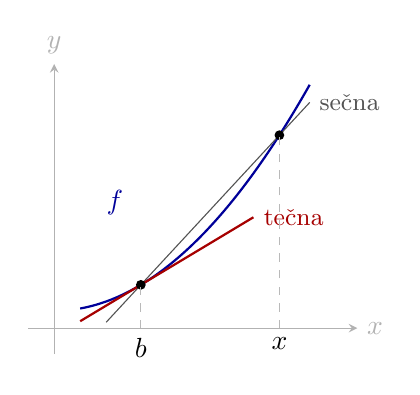
\begin{tikzpicture}[scale=1.1,>=stealth]
  \draw[->,gray!60](-0.3,0)--(3.5,0) node[right]{$x$};
  \draw[->,gray!60](0,-0.3)--(0,3.05) node[above]{$y$};
  \draw[blue!60!black,thick,domain=0.3:2.95,smooth,samples=60] plot(\x,{0.3*\x*\x+0.2});
  \node[blue!60!black] at (0.7,1.45){$f$};
  \draw[gray!65!black] (0.6,0.068)--(2.95,2.606) node[right]{\small sečna};
  \draw[red!65!black,thick] (0.3,0.08)--(2.3,1.28) node[right]{\small tečna};
  \fill (1,0.5) circle(1.6pt); \fill (2.6,2.228) circle(1.6pt);
  \draw[dashed,gray!55](1,0)--(1,0.5); \draw[dashed,gray!55](2.6,0)--(2.6,2.228);
  \node[below] at (1,0){$b$}; \node[below] at (2.6,0){$x$};
\end{tikzpicture}\obrpopis{Derivace jako směrnice tečny: pro $f(x)=0{,}3\,x^2+0{,}2$ a $b=1$ je $f(b)=0{,}5$, $f(2{,}6)=2{,}228$; směrnice sečny $\frac{2{,}228-0{,}5}{2{,}6-1}=1{,}08$ se při $x\to b$ blíží směrnici tečny $f'(b)=0{,}6\,b=0{,}6$.}
\end{center}

\begin{veta}[Diferencovatelnost $\Rightarrow$ spojitost]
Má-li $f$ v $b$ vlastní derivaci, je v $b$ spojitá. (Opak neplatí: $|x|$ je v $0$ spojitá, ale nemá tam derivaci.)
\end{veta}

\begin{veta}[Pravidla pro derivování]
Mají-li $f,g$ v $b$ derivaci (vlastní či nevlastní) a je-li pravá strana definovaná, platí
\[
  (f+g)'=f'+g',\quad (\alpha f)'=\alpha f',\quad (fg)'=f'g+fg'\ \text{(Leibniz)},\quad \Big(\tfrac{f}{g}\Big)'=\frac{f'g-fg'}{g^2}\ (g(b)\neq0).
\]
U součinu musí být navíc $f$ nebo $g$ v $b$ spojitá, u podílu $g$ spojitá v $b$. (Je-li derivace vlastní, spojitost plyne z předchozí věty, takže u vlastních derivací je předpoklad splněn automaticky.)
Dále \emph{řetízkové pravidlo} pro složenou funkci: $(f\circ g)'(a)=f'(g(a))\cdot g'(a)$, a pravidlo pro inverzní funkci: $(f^{-1})'(y_0)=\dfrac{1}{f'(x_0)}$, kde $y_0=f(x_0)$ a $f'(x_0)\neq0$.
\end{veta}

\begin{poznamka}[Derivace elementárních funkcí]
$(x^n)'=nx^{n-1}$, $(\exp x)'=\exp x$, $(\ln x)'=\tfrac1x$, $(\sin x)'=\cos x$, $(\cos x)'=-\sin x$, $(\arctan x)'=\tfrac1{1+x^2}$. Vyjde-li na pravé straně pravidel neurčitý výraz (např. $(+\infty)\cdot0$), o derivaci vlevo nic neplyne. A i když neurčitý výraz nevyjde, bez ověření spojitosti lze dostat chybný výsledek: pro $f=g=\tfrac1{10}+\mathrm{sgn}\,x$ dá Leibnizův vzorec v~$0$ zdánlivě $+\infty$, ve skutečnosti ale $fg$ v~$0$ derivaci nemá (jednostranné derivace jsou $+\infty$ a $-\infty$).
\end{poznamka}

\video{https://www.youtube.com/watch?v=9vKqVkMQHKk}{3Blue1Brown, \emph{Essence of Calculus} kap.~2 -- \emph{The paradox of the derivative} (co je derivace; navazují kap.~3--4: vzorce geometricky, řetízkové a~součinové pravidlo).}

\video{https://www.youtube.com/watch?v=m2MIpDrF7Es}{3Blue1Brown, \emph{Essence of Calculus} kap.~5 -- \emph{What's so special about Euler's number e?} (proč $(\exp x)'=\exp x$ a~odkud se bere~$e$).}

\subsection{l'Hospitalovo pravidlo}

\begin{veta}[l'Hospitalovo pravidlo]
Nechť $a\in\mathbb{R}^*$, funkce $f,g$ mají na prstencovém okolí $P(a,\delta)$ vlastní derivaci a $g'\neq0$. Je-li splněno
\begin{enumerate}
  \item $\lim_{x\to a}f(x)=\lim_{x\to a}g(x)=0$, \quad nebo \quad
  \item $\lim_{x\to a}|g(x)|=+\infty$,
\end{enumerate}
a existuje-li $\lim_{x\to a}\dfrac{f'(x)}{g'(x)}=A\in\mathbb{R}^*$, pak i $\lim_{x\to a}\dfrac{f(x)}{g(x)}=A$.
\end{veta}

\begin{poznamka}
Pravidlo řeší jen neurčité výrazy $\tfrac00$ a $\tfrac{\infty}{\infty}$. Pokud předpoklad neplatí (čitatel a jmenovatel nejdou oba k nule ani k nekonečnu), je jeho použití \emph{chybné}. Také: pokud $\lim f'/g'$ \emph{neexistuje}, pravidlo neříká nic (limita $f/g$ může přesto existovat).
\end{poznamka}

\begin{priklad}[Správné použití l'Hospitala]
\textbf{Zadání.} Spočítejte $\lim_{x\to0}\dfrac{\sin x-x}{x^3}$.\par
\textbf{Řešení.}
\[
  \lim_{x\to0}\frac{\sin x-x}{x^3}
  \overset{0/0}{=}\lim_{x\to0}\frac{\cos x-1}{3x^2}
  \overset{0/0}{=}\lim_{x\to0}\frac{-\sin x}{6x}=-\frac16.
\]
\end{priklad}

\subsection{Vyšetření průběhu funkce}

Derivace jsou hlavním nástrojem pro určení monotonie, extrémů a konvexity, z nichž lze sestavit náčrt grafu.

\begin{veta}[Nutná podmínka lokálního extrému]
Nabývá-li $f$ v bodě $a$ lokálního extrému a má tam derivaci, je $f'(a)=0$. Ekvivalentně (kontrapozicí): má-li $f$ v $a$ nenulovou derivaci $f'(a)\neq0$, pak v $a$ lokální extrém \emph{nemá}. Lokální extrém tedy může nastat jen tam, kde $f'(a)=0$ nebo kde derivace neexistuje (např. v krajních bodech intervalu).
\end{veta}

\begin{veta}[Derivace a monotonie]
Nechť $f$ je spojitá na intervalu $J$ a má derivaci v jeho vnitřních bodech. Je-li $f'>0$ na vnitřku $J$, je $f$ na $J$ rostoucí; je-li $f'<0$, je klesající (s $\ge,\le$ obdobně neklesající/nerostoucí). Je-li $f'\equiv0$, je $f$ konstantní.
\end{veta}

\begin{definice}[Konvexita a konkavita]
Funkce $f$ je na intervalu $I$ \emph{konvexní}, leží-li její graf na každém podintervalu pod úsečkou spojující krajní body grafu, tj. pro $a<x<b$ z $I$
\[
  f(x)\le f(a)+(x-a)\frac{f(b)-f(a)}{b-a};
\]
\emph{konkávní} je při opačné nerovnosti (graf nad úsečkou). U ostrých nerovností mluvíme o ryzí konvexitě/konkavitě.
\end{definice}

\begin{center}
\begin{minipage}[t]{0.48\linewidth}\centering
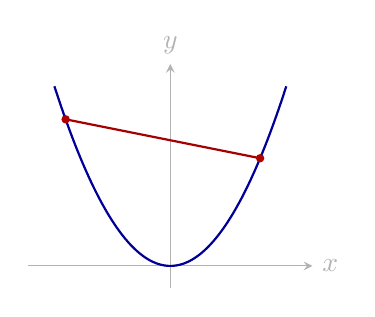
\begin{tikzpicture}[scale=0.95,>=stealth]
  \draw[->,gray!60](-1.9,0)--(1.9,0) node[right]{$x$};
  \draw[->,gray!60](0,-0.3)--(0,2.7) node[above]{$y$};
  \draw[blue!60!black,thick,domain=-1.55:1.55,smooth,samples=60] plot(\x,{\x*\x});
  \draw[red!65!black,thick] (-1.4,1.96)--(1.2,1.44);
  \fill[red!70!black] (-1.4,1.96) circle(1.6pt);
  \fill[red!70!black] (1.2,1.44) circle(1.6pt);
\end{tikzpicture}\\[0.2em]
{\small konvexní: tětiva nad grafem}
\end{minipage}\hfill
\begin{minipage}[t]{0.48\linewidth}\centering
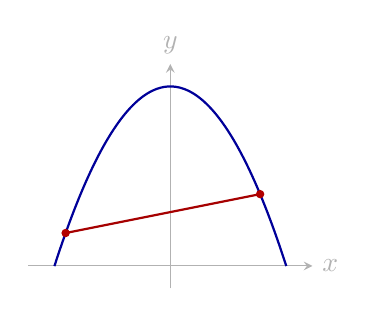
\begin{tikzpicture}[scale=0.95,>=stealth]
  \draw[->,gray!60](-1.9,0)--(1.9,0) node[right]{$x$};
  \draw[->,gray!60](0,-0.3)--(0,2.7) node[above]{$y$};
  \draw[blue!60!black,thick,domain=-1.55:1.55,smooth,samples=60] plot(\x,{2.4-\x*\x});
  \draw[red!65!black,thick] (-1.4,0.44)--(1.2,0.96);
  \fill[red!70!black] (-1.4,0.44) circle(1.6pt);
  \fill[red!70!black] (1.2,0.96) circle(1.6pt);
\end{tikzpicture}\\[0.2em]
{\small konkávní: tětiva pod grafem}
\end{minipage}
\end{center}

\begin{veta}[Druhá derivace a konvexita]
Má-li $f$ na otevřeném intervalu $I$ druhou derivaci, pak: $f''>0$ na $I$ $\Rightarrow$ $f$ je ryze konvexní; $f''<0$ $\Rightarrow$ ryze konkávní. Bod, kde graf přechází z jedné strany tečny na druhou (mění se konvexita/konkavita), je \emph{inflexní bod}.
\end{veta}

\begin{poznamka}[Rolleova a Lagrangeova věta]
Na pozadí těchto tvrzení stojí věty o střední hodnotě. \emph{Rolleova}: je-li $f$ spojitá na $[a,b]$, má derivaci na $(a,b)$ a $f(a)=f(b)$, existuje $c\in(a,b)$ s $f'(c)=0$. \emph{Lagrangeova}: za týchž předpokladů (bez $f(a)=f(b)$) existuje $c$ s $f'(c)=\tfrac{f(b)-f(a)}{b-a}$ -- tj. někde je tečna rovnoběžná se sečnou koncových bodů.
\end{poznamka}

\begin{priklad}[Vyšetření průběhu]
\textbf{Zadání.} Vyšetřete průběh $f(x)=x^3-3x$ na $\mathbb{R}$.

\textbf{Řešení.}
Funkce je lichá, spojitá, $\lim_{x\to\pm\infty}f=\pm\infty$.\par
\textbf{Monotonie a extrémy.} $f'(x)=3x^2-3=3(x-1)(x+1)$, takže $f'>0$ na $(-\infty,-1)$ i $(1,\infty)$ (rostoucí) a $f'<0$ na $(-1,1)$ (klesající). V $x=-1$ je proto lokální maximum $f(-1)=2$, v $x=1$ lokální minimum $f(1)=-2$.\par
\textbf{Konvexita.} $f''(x)=6x$, tedy $f$ je konkávní na $(-\infty,0)$ a konvexní na $(0,\infty)$; v $x=0$ je inflexní bod ($f(0)=0$).
\begin{center}
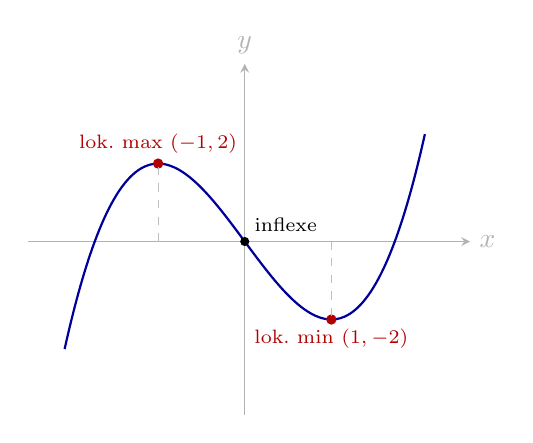
\begin{tikzpicture}[scale=1.1,>=stealth]
  \draw[->,gray!60](-2.5,0)--(2.6,0) node[right]{$x$};
  \draw[->,gray!60](0,-2.0)--(0,2.05) node[above]{$y$};
  \draw[blue!60!black,thick,domain=-2.08:2.08,smooth,samples=90] plot(\x,{0.45*(\x*\x*\x-3*\x)});
  \fill[red!70!black] (-1,0.9) circle(1.7pt) node[above]{\scriptsize lok.\ max $(-1,2)$};
  \fill[red!70!black] (1,-0.9) circle(1.7pt) node[below]{\scriptsize lok.\ min $(1,-2)$};
  \fill[black] (0,0) circle(1.5pt) node[above right]{\scriptsize inflexe};
  \draw[dashed,gray!50](-1,0)--(-1,0.9); \draw[dashed,gray!50](1,0)--(1,-0.9);
\end{tikzpicture}\obrpopis{Průběh $f(x)=x^3-3x$: $f'(x)=3x^2-3$, kořeny $\pm 1$ ($f'(\pm 1)=0$) odpovídají lokálním extrémům $f(-1)=2$, $f(1)=-2$; $f''(0)=0$ je inflexní bod (svislé měřítko zhuštěno).}
\end{center}
\end{priklad}

\subsection{Taylorův polynom (limitní forma)}

Tečna je nejlepší aproximace přímkou. Taylorův polynom je analogická nejlepší aproximace polynomem stupně~$n$.

\begin{definice}[Taylorův polynom]
Má-li $f$ v bodě $a$ vlastní $n$-tou derivaci, je \emph{Taylorův polynom řádu $n$} funkce $f$ v $a$ roven
\[
  T_n^{f,a}(x)=\sum_{i=0}^{n}\frac{f^{(i)}(a)}{i!}(x-a)^i
  =f(a)+f'(a)(x-a)+\frac{f''(a)}{2!}(x-a)^2+\cdots+\frac{f^{(n)}(a)}{n!}(x-a)^n.
\]
\end{definice}

\begin{veta}[Charakterizace Taylorova polynomu -- limitní forma]
$T_n^{f,a}(x)$ je \emph{jediný} polynom stupně nejvýše $n$, pro který platí
\[
  \lim_{x\to a}\frac{f(x)-T_n^{f,a}(x)}{(x-a)^n}=0,
\]
což zapisujeme též $f(x)=T_n^{f,a}(x)+o(|x-a|^n)$ pro $x\to a$.
\end{veta}

\begin{intuice}
Taylorův polynom \uv{kopíruje} funkci v bodě $a$ až do $n$-té derivace ($T^{(i)}(a)=f^{(i)}(a)$). Zbytek $f-T_n$ klesá k nule rychleji než $(x-a)^n$ -- proto je $T_n$ nejlepší možná aproximace polynomem daného stupně. Maclaurinovy rozvoje (se středem $0$): $\exp x=\sum \tfrac{x^n}{n!}$, $\sin x=x-\tfrac{x^3}{3!}+\cdots$, $\cos x=1-\tfrac{x^2}{2!}+\cdots$, $\ln(1+x)=x-\tfrac{x^2}{2}+\tfrac{x^3}{3}-\cdots$
\end{intuice}

\begin{center}
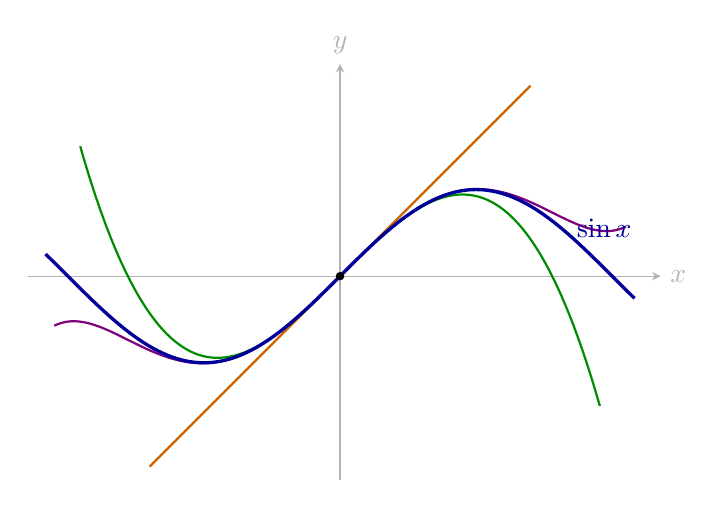
\begin{tikzpicture}[scale=1.1,>=stealth]
  \draw[->,gray!60](-3.6,0)--(3.7,0) node[right]{$x$};
  \draw[->,gray!60](0,-2.35)--(0,2.45) node[above]{$y$};
  % T1(x) = x
  \draw[orange!80!black,thick,domain=-2.2:2.2,smooth,samples=2] plot(\x,{\x});
  % T3(x) = x - x^3/6  (omezeno aby neuteklo)
  \draw[green!55!black,thick,domain=-3.0:3.0,smooth,samples=80] plot(\x,{\x-(\x*\x*\x)/6});
  % T5(x) = x - x^3/6 + x^5/120
  \draw[violet,thick,domain=-3.3:3.3,smooth,samples=90] plot(\x,{\x-(\x*\x*\x)/6+(\x*\x*\x*\x*\x)/120});
  % sin x
  \draw[blue!60!black,very thick,domain=-3.4:3.4,smooth,samples=90] plot(\x,{sin(deg(\x))});
  \node[blue!60!black] at (3.05,0.55){$\sin x$};
  \fill (0,0) circle(1.4pt);
\end{tikzpicture}\obrpopis{%
Taylorovy polynomy $\sin x$ kolem středu $0$:
{\color{orange!80!black}$T_1(x)=x$} (oranžová),
{\color{green!55!black}$T_3(x)=x-\tfrac{x^3}{6}$} (zelená),
{\color{violet}$T_5(x)=x-\tfrac{x^3}{6}+\tfrac{x^5}{120}$} (fialová).
Vyšší stupeň dává lepší shodu se {\color{blue!60!black}$\sin x$} v~okolí středu; na krajích se každý polynom nakonec rozejde.}
\end{center}

\begin{poznamka}
Velikost chyby udává \emph{Lagrangeův tvar zbytku}: $f(x)-T_n^{f,a}(x)=\tfrac{f^{(n+1)}(c)}{(n+1)!}(x-a)^{n+1}$ pro nějaké $c$ mezi $a$ a $x$. Taylorův polynom také usnadňuje výpočet limit typu $\tfrac00$: čitatel i jmenovatel se nahradí rozvojem dostatečného řádu (často méně pracné než opakovaný l'Hospital).
\end{poznamka}

\begin{priklad}[Limita přes Taylorův polynom]
\textbf{Zadání.} Spočítejte $\lim_{x\to0}\dfrac{\sin x-x}{x^3}$ pomocí Taylorova rozvoje.\par
\textbf{Řešení.} Z $\sin x=x-\tfrac{x^3}{6}+o(x^3)$ plyne $\sin x-x=-\tfrac{x^3}{6}+o(x^3)$, takže
\[
  \lim_{x\to0}\frac{\sin x-x}{x^3}=\lim_{x\to0}\frac{-\tfrac{x^3}{6}+o(x^3)}{x^3}=-\frac16.
\]
Stačil jeden rozvoj místo trojího derivování.
\end{priklad}

\video{https://www.youtube.com/watch?v=3d6DsjIBzJ4}{3Blue1Brown, \emph{Essence of Calculus} kap.~11 -- \emph{Taylor series} (Taylorovy řady vizuálně).}

% ============================================================
\section{Integrály a jejich aplikace}

Integrování je v jistém smyslu opačná operace k derivování: ze známé \uv{rychlosti} (derivace) rekonstruujeme funkci. Z toho vyrůstá výpočet ploch, objemů a odhadů součtů.

\subsection{Primitivní funkce a metody výpočtu}

\begin{definice}[Primitivní funkce]
Nechť $f$ je definovaná na otevřeném intervalu $I$. Funkce $F$ je \emph{primitivní funkcí} k $f$ na $I$, pokud $F'(x)=f(x)$ pro každé $x\in I$. Množinu primitivních funkcí značíme $\int f(x)\,\mathrm{d}x$.
\end{definice}

\begin{veta}[Jednoznačnost až na konstantu]
Je-li $F$ primitivní k $f$ na intervalu $I$, jsou primitivními funkcemi právě všechny funkce $F+c$, $c\in\mathbb{R}$. (Dvě primitivní funkce se liší o konstantu.) Každá spojitá funkce na otevřeném intervalu primitivní funkci má.
\end{veta}

Univerzální vzorec pro primitivní funkci součinu nebo podílu neexistuje; dvě základní techniky pocházejí z pravidel pro derivování složené funkce a součinu.

\begin{veta}[Substituce a per partes]
Nechť uvažované funkce jsou spojité. Pak:
\[
  \text{(substituce)}\quad \int f(\varphi(t))\,\varphi'(t)\,\mathrm{d}t=F(\varphi(t))+c,\qquad\text{kde } F=\int f,
\]
\[
  \text{(per partes)}\quad \int f(x)G(x)\,\mathrm{d}x=F(x)G(x)-\int F(x)g(x)\,\mathrm{d}x,
\]
kde $F$ je primitivní k $f$ a $G$ primitivní k $g$.
\end{veta}

\begin{intuice}
\emph{Substituce} čte řetízkové pravidlo pozpátku (\uv{$\varphi'(t)\,\mathrm{d}t$} se schová do \uv{$\mathrm{d}x$}). \emph{Per partes} čte pozpátku Leibnizovo pravidlo $(FG)'=fG+Fg$: jednu funkci derivujeme, druhou integrujeme, výhodné když se tím integrál zjednoduší.
\end{intuice}

\begin{priklad}[Substituce]
\textbf{Zadání.} Spočítejte $\int x\,e^{x^2}\,\mathrm{d}x$.\par
\textbf{Řešení.} Volbou $t=x^2$ máme $\mathrm{d}t=2x\,\mathrm{d}x$, tedy $x\,\mathrm{d}x=\tfrac12\,\mathrm{d}t$:
\[
  \int x\,e^{x^2}\,\mathrm{d}x=\tfrac12\int e^{t}\,\mathrm{d}t=\tfrac12 e^{t}+c=\tfrac12 e^{x^2}+c.
\]
U \emph{určitého} integrálu navíc přepočítáme meze dosazením do $t=\varphi(x)$, takže se není nutné vracet k~původní proměnné.
\end{priklad}

\begin{priklad}[SZZ léto 2022 č.~3: Integrace per partes, $\int x\sin x$] \szzotazka{léto 2022}{3}{Integrál (per partes)}\par
\textbf{Zadání.} Nechť $I\subseteq\mathbb{R}$ je neprázdný otevřený interval. (1)~Jaký je vztah mezi dvěma primitivními funkcemi k~téže funkci na~$I$? Zdůvodněte. (2)~Pro $f,g\colon I\to\mathbb{R}$ s~primitivními funkcemi $F,G$ napište vzorec pro primitivní funkci k~$fG$, známe-li primitivní funkci k~$Fg$. (3)~Podle tohoto vzorce najděte primitivní funkci k~$f(x)=x\sin x$.\par
\textbf{Řešení.}
\begin{enumerate}
  \item Dvě primitivní funkce k~téže funkci na intervalu se liší o~konstantu: jsou-li $F_1,F_2$ obě primitivní k~$f$, má $F_1-F_2$ na~$I$ nulovou derivaci, je tedy konstantní.
  \item Z~Leibnizova pravidla $(FG)'=fG+Fg$ integrací plyne per partes
    \[
      \int f(x)G(x)\,\mathrm{d}x=F(x)G(x)-\int F(x)g(x)\,\mathrm{d}x,
    \]
    tj.\ primitivní k~$fG$ je $F\cdot G$ mínus primitivní k~$Fg$.
  \item Volíme $F=x$ ($f=1$) a~$G=-\cos x$ ($g=\sin x$); pak $fG=-\cos x$ a~$Fg=x\sin x$. Ze vzorce $\int(-\cos x)\,\mathrm{d}x=x(-\cos x)-\int x\sin x\,\mathrm{d}x$, tj.\ $-\sin x=-x\cos x-\int x\sin x\,\mathrm{d}x$, odkud
    \[
      \int x\sin x\,\mathrm{d}x=\sin x-x\cos x+C.
    \]
    (Ověření: $(\sin x-x\cos x)'=\cos x-(\cos x-x\sin x)=x\sin x$.)
\end{enumerate}
\end{priklad}

\video{https://www.youtube.com/watch?v=rfG8ce4nNh0}{3Blue1Brown, \emph{Essence of Calculus} kap.~8 -- \emph{Integration and the fundamental theorem of calculus} (integrál a~jeho souvislost s~derivací).}

\subsection{Určitý integrál: Newtonův a Riemannův}

Existují dvě cesty k určitému integrálu. \emph{Newtonův} stojí na primitivní funkci, \emph{Riemannův} na ploše pod grafem; za rozumných předpokladů dávají totéž.

\begin{definice}[Newtonův integrál]
Má-li $f$ na $(a,b)$ primitivní funkci $F$ s vlastními jednostrannými limitami $F(a^+)=\lim_{x\to a^+}F$ a $F(b^-)=\lim_{x\to b^-}F$, definujeme
\[
  (N)\!\int_a^b f(x)\,\mathrm{d}x:=[F]_a^b=F(b^-)-F(a^+).
\]
Definice nezávisí na volbě $F$ (liší se jen o konstantu). Třídu funkcí, které mají na $(a,b)$ Newtonův integrál, značíme $N(a,b)$.
\end{definice}

\begin{definice}[Riemannův integrál]
\emph{Dělením} intervalu $[a,b]$ je $D=(a_0,\dots,a_k)$ s $a=a_0<\dots<a_k=b$; klade intervaly $I_i=[a_i,a_{i+1}]$. \emph{Dolní} a \emph{horní Riemannova suma} jsou
\[
  s(f,D)=\sum_i |I_i|\,m_i,\qquad S(f,D)=\sum_i |I_i|\,M_i,\qquad m_i=\inf_{I_i}f,\ M_i=\sup_{I_i}f.
\]
\emph{Dolní} a \emph{horní integrál} jsou $\underline{\int}_a^b f=\sup_D s(f,D)$ a $\overline{\int}_a^b f=\inf_D S(f,D)$. Pokud se rovnají a jsou konečné, jejich společnou hodnotu nazýváme \emph{Riemannovým integrálem} $\int_a^b f$. Třídu riemannovsky integrovatelných funkcí na $[a,b]$ značíme $R[a,b]$.
\end{definice}

\begin{intuice}
Riemannův integrál formalizuje obsah plochy pod grafem: zdola ji odhadujeme \uv{schody} pod grafem (dolní sumy), shora \uv{schody} nad grafem (horní sumy). Když lze rozdíl horní a dolní sumy učinit libovolně malým, oba odhady splynou a definují obsah. (Funkce musí být omezená; např. Dirichletova funkce integrovatelná není.)
\end{intuice}

\begin{center}
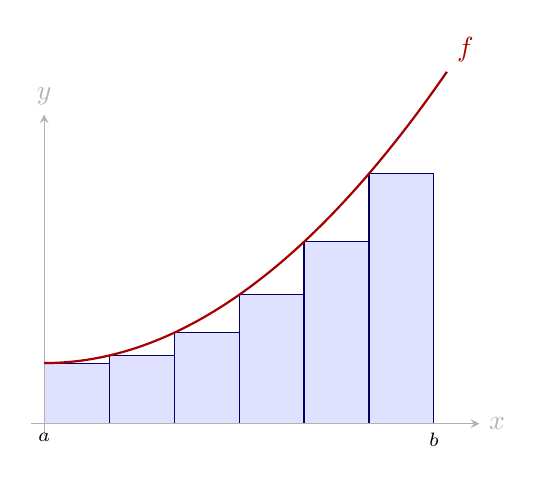
\begin{tikzpicture}[x=1.65cm,y=1.54cm,>=stealth]
  \foreach \i in {0,...,5}{
    \pgfmathsetmacro\xa{\i*0.5}
    \pgfmathsetmacro\h{0.25*\xa*\xa+0.5}
    \fill[blue!12] (\xa,0) rectangle (\xa+0.5,\h);
    \draw[blue!40!black,thin] (\xa,0) rectangle (\xa+0.5,\h);
  }
  \draw[->,gray!60](-0.1,0)--(3.35,0) node[right]{$x$};
  \draw[->,gray!60](0,-0.1)--(0,2.55) node[above]{$y$};
  \draw[red!65!black,thick,domain=0:3.1,smooth,samples=60] plot(\x,{0.25*\x*\x+0.5}) node[above right]{$f$};
  \node[below] at (0,0){\scriptsize$a$}; \node[below] at (3,0){\scriptsize$b$};
\end{tikzpicture}\obrpopis{Dolní Riemannova suma pro $f(x)=0{,}25\,x^2+0{,}5$ na $[a,b]=[0,3]$ s~dělením $\Delta x=0{,}5$ (6 obdélníků): výšky v~levých krajích, neboť $f$ roste. Horní suma by použila pravé kraje; zjemňováním dělení ($\Delta x\to 0$) se obě sumy sevřou k~obsahu pod grafem.}
\end{center}

\begin{veta}[Postačující podmínky integrovatelnosti]
Je-li $f$ na $[a,b]$ spojitá, nebo je-li na $[a,b]$ monotónní, pak má na $[a,b]$ Riemannův integrál.
\end{veta}

\subsection{Souvislost s primitivní funkcí (základní věty analýzy)}

\begin{veta}[1.\ základní věta analýzy]
Nechť $f\in R[a,b]$ a $F(x)=\int_a^x f(t)\,\mathrm{d}t$. Pak $F$ je na $[a,b]$ spojitá a v každém bodě $x_0$, kde je $f$ spojitá, platí $F'(x_0)=f(x_0)$. Speciálně každá spojitá funkce má primitivní funkci.
\end{veta}

\begin{veta}[2.\ základní věta analýzy]
Existují-li oba integrály, jsou si rovny: pro $f\in R[a,b]\cap N(a,b)$ platí
\[
  \int_a^b f=(N)\!\int_a^b f=[F]_a^b=F(b)-F(a).
\]
Proto u určitého integrálu obvykle nerozlišujeme, zda jde o Newtonův či Riemannův. Spojité funkce mají oba a shodují se.
\end{veta}

\begin{intuice}
Derivování a integrování jsou navzájem inverzní operace: derivace \uv{rozbalí} plochu naakumulovanou funkcí ($F'=f$), zatímco určitý integrál \uv{naakumuluje} hodnoty $f$ a výsledek je rozdíl primitivní funkce v krajních bodech. To je obsah obou základních vět.
\end{intuice}

\video{https://www.youtube.com/watch?v=FnJqaIESC2s}{3Blue1Brown, \emph{Essence of Calculus} kap.~9 -- \emph{What does area have to do with slope?} (intuice za základními větami analýzy: plocha $\leftrightarrow$ směrnice).}

\subsection{Aplikace integrálů}

\paragraph{Obsahy rovinných útvarů.} Obsah útvaru pod grafem nezáporné funkce $f$ na $[a,b]$ je přímo $\int_a^b f(x)\,\mathrm{d}x$.

\begin{priklad}[SZZ podzim 2024 č.~3: Integrály a primitivní funkce] \szzotazka{podzim 2024}{3}{Integrály a primitivní funkce}\par
\textbf{Zadání.} Spočítejte obsah útvaru pod grafem $f(x)=x\cos x$ pro $x\in[0,\tfrac\pi2]$.\par
\textbf{Řešení.} Obsah je $\int_0^{\pi/2}x\cos x\,\mathrm{d}x$. Per partes volíme $f=\cos x$, $G=x$ (tedy $F=\sin x$, $g=G'=1$), takže $\int fG=FG-\int Fg$:
\[
  \int_0^{\pi/2}x\cos x\,\mathrm{d}x=\big[x\sin x\big]_0^{\pi/2}-\int_0^{\pi/2}\sin x\,\mathrm{d}x=\frac\pi2-\big[-\cos x\big]_0^{\pi/2}=\frac\pi2-1.
\]

\begin{center}
\begin{tikzpicture}[x=2.2cm,y=2.2cm,>=stealth]
  % vyplnena plocha pod krivkou f(x)=x cos x na [0, pi/2]
  \fill[blue!12,domain=0:1.5708,smooth,samples=80]
        plot(\x,{\x*cos(deg(\x))}) -- (1.5708,0) -- (0,0) -- cycle;
  \draw[->,gray!60](-0.1,0)--(1.95,0) node[right]{$x$};
  \draw[->,gray!60](0,-0.1)--(0,0.85) node[above]{$y$};
  \draw[blue!60!black,thick,domain=0:1.5708,smooth,samples=80]
        plot(\x,{\x*cos(deg(\x))});
  \node[blue!60!black] at (0.62,0.66){\small $f(x)=x\cos x$};
  \node[below] at (0,0){\scriptsize $0$};
  \draw[dotted,gray!55] (1.5708,0)--(1.5708,0.02);
  \node[below] at (1.5708,0){\scriptsize $\tfrac\pi2$};
\end{tikzpicture}\obrpopis{%
Vyznačená plocha pod grafem $f(x)=x\cos x$ na $[0,\tfrac\pi2]$ se rovná hodnotě integrálu $\int_0^{\pi/2}x\cos x\,\mathrm{d}x=\tfrac\pi2-1\approx0{,}571$.}
\end{center}
\end{priklad}

\begin{priklad}[SZZ podzim 2025 č.~3: Základy analýzy] \szzotazka{podzim 2025}{3}{Základy analýzy}\par
\textbf{Zadání.}
Útvar $U_p$ ($p>0$) je ohraničen přímkami $x=p$, $x=p+1$, osou $x$ a~grafem $f(x)=x+\tfrac1x$.
\begin{enumerate}[label=(\arabic*)]
  \item Ukažte, že má obsah $p+\ln(1+\tfrac1p)+\tfrac12$.
  \item Existuje $p\in(0,100)$ s~obsahem větším než $10\,000$?
  \item Najděte $p$, pro něž je obsah minimální.
\end{enumerate}

\textbf{Řešení.}
\begin{enumerate}[label=(\arabic*)]
  \item \textbf{Primitivní funkce a dosazení mezí.} Obsah je $u(p)=\int_p^{p+1}\big(x+\tfrac1x\big)\,\mathrm{d}x$; s~primitivní funkcí $\tfrac{x^2}{2}+\ln x$:
    \[
      u(p)=\Big[\tfrac{x^2}{2}+\ln x\Big]_p^{p+1}=\frac{(p+1)^2-p^2}{2}+\ln\frac{p+1}{p}=p+\tfrac12+\ln\!\big(1+\tfrac1p\big).
    \]
  \item \textbf{Limita pro $p\to0^+$.} Pro $p\to0^+$ je $\ln(1+\tfrac1p)\to+\infty$, takže $u(p)\to+\infty$; na dostatečně malém $p>0$ (a~tedy i~v~$(0,100)$) obsah přesáhne libovolnou mez, speciálně $10\,000$.
  \item \textbf{Derivace a kritický bod.} Řetízkové pravidlo na $\ln(1+\tfrac1p)$ dává
    \[ u'(p)=1+\dfrac{-1/p^2}{1+1/p}=1-\dfrac{1}{p^2+p}. \]
    Z~$u'(p)=0$ plyne $p^2+p-1=0$ s~jediným kladným kořenem $p_0=\tfrac{-1+\sqrt5}{2}$.\par
    \textbf{Konvexita.} $u''(p)=\dfrac{2p+1}{(p^2+p)^2}>0$, takže $u$ je ryze konvexní a $p_0$ je bodem globálního minima:
    \[
      p_0=\tfrac{-1+\sqrt5}{2}.
    \]
    (Příklad pěkně spojuje integrál (obsah) s~derivací (extrém).)
\end{enumerate}
\end{priklad}

\paragraph{Odhady součtů řad.} Vztah mezi integrálem a Riemannovými sumami dává odhady konečných i nekonečných součtů.

\begin{veta}[Odhad sumy integrálem a integrální kritérium]
Je-li $f$ neklesající na $[1,n]$, platí $\sum_{k=1}^{n-1}f(k)\le\int_1^n f\le\sum_{k=2}^{n}f(k)$ (pro nerostoucí $f$ se nerovnosti obrátí). Důsledek pro nezápornou nerostoucí $f:[1,\infty)\to[0,\infty)$: řada $\sum_{k\ge1}f(k)$ konverguje právě tehdy, když $\lim_{b\to\infty}\int_1^b f<+\infty$.
\end{veta}

\begin{poznamka}
Zápis $\int_1^\infty f:=\lim_{b\to\infty}\int_1^b f$ (pokud limita vpravo existuje) se nazývá \emph{nevlastní integrál} -- rozšiřuje integrál na neohraničený interval. V~tomto tvaru ho používáme v~kritériu výše i~v~příkladu níže.
\end{poznamka}

\begin{intuice}
Každý člen $f(k)$ je výška obdélníku o~šířce~$1$; u monotónní $f$ tyto obdélníky integrál $\int_1^n f$ sevřou zdola i shora podle toho, bereme-li jako výšku levý, či pravý krajní bod intervalu. Posláním $n\to\infty$ odtud plyne integrální kritérium: nezáporná nerostoucí řada konverguje právě tehdy, když konverguje příslušný nevlastní integrál.
\end{intuice}

\begin{priklad}[Harmonická čísla a divergence]
\textbf{Zadání.} Pomocí odhadu sumy integrálem rozhodněte o konvergenci řad $\sum_{k\ge1}\tfrac1k$ a $\sum_{k\ge1}\tfrac1{k^s}$ (pro $s>1$).\par
\textbf{Řešení.} Pro $f(x)=\tfrac1x$ dává odhad $\ln n+\tfrac1n\le H_n\le \ln n+1$, kde $H_n=1+\tfrac12+\dots+\tfrac1n$. Protože $\ln n\to+\infty$, harmonická řada $\sum\tfrac1k$ diverguje. Naopak $\int_1^\infty x^{-s}\,\mathrm{d}x=\tfrac1{s-1}<\infty$ pro $s>1$, takže $\sum\tfrac1{k^s}$ pro $s>1$ konverguje.
\end{priklad}

\paragraph{Objemy a povrchy rotačních těles; délka křivky.} Má-li $f$ na $[a,b]$ spojitou derivaci a $f\ge0$, pak pro těleso vzniklé rotací útvaru pod grafem kolem osy $x$ platí
\[
  \text{objem}=\pi\int_a^b f(t)^2\,\mathrm{d}t,\qquad
  \text{povrch}=2\pi\int_a^b f(t)\sqrt{1+(f'(t))^2}\,\mathrm{d}t,
\]
a délka grafu (oblouku) funkce $f$ je
\[
  \text{délka}=\int_a^b \sqrt{1+(f'(t))^2}\,\mathrm{d}t.
\]

\begin{intuice}
Všechny tři vzorce vznikají \uv{nasekáním} útvaru na tenké plátky a sečtením (limitou) jejich příspěvků: objem jako součet tenkých válečků o poloměru $f(x)$ ($\pi f(x)^2\,\mathrm{d}x$), délka křivky jako součet maličkých přepon $\sqrt{1+(f')^2}\,\mathrm{d}x$ (Pythagoras na přírůstky $\mathrm{d}x$ a $f'(x)\,\mathrm{d}x$).
\end{intuice}

\begin{priklad}[Objem koule]
\textbf{Zadání.} Odvoďte integrálem vzorec pro objem koule o~poloměru $r$.

\textbf{Řešení.}\par
\textbf{Volba rotující funkce.} Koule o~poloměru $r$ vznikne rotací horního půlkruhu pod grafem $f(x)=\sqrt{r^2-x^2}$ (horní půlkružnice o~poloměru $r$) na $[-r,r]$ kolem osy~$x$. Řez kolmý k~ose~$x$ v~bodě $x$ je kruh o~poloměru $f(x)$, tedy o~obsahu $\pi f(x)^2$.\par
\textbf{Integrace.} Objem je součet (integrál) tenkých plátků o~tloušťce $\mathrm{d}x$:
\[
  V=\pi\int_{-r}^{r} f(x)^2\,\mathrm{d}x
   =\pi\int_{-r}^{r}\big(\sqrt{r^2-x^2}\big)^2\,\mathrm{d}x
   =\pi\int_{-r}^{r}(r^2-x^2)\,\mathrm{d}x
   =\pi\Big[r^2x-\tfrac{x^3}{3}\Big]_{-r}^{r}.
\]
Druhá mocnina zrušila odmocninu a zbyl polynom (zde je $r$ konstanta); jeho primitivní funkce je $r^2x-\tfrac{x^3}{3}$.\par
\textbf{Dosazení mezí.} V~horní $r^2\!\cdot\!r-\tfrac{r^3}{3}=r^3-\tfrac{r^3}{3}=\tfrac23 r^3$, v~dolní $r^2\!\cdot\!(-r)-\tfrac{(-r)^3}{3}=-r^3+\tfrac{r^3}{3}=-\tfrac23 r^3$. Jejich rozdíl je $\tfrac23 r^3-\big(-\tfrac23 r^3\big)=\tfrac43 r^3$, a tedy
\[
  V=\pi\cdot\tfrac43 r^3=\frac{4}{3}\pi r^3.
\]

\begin{center}
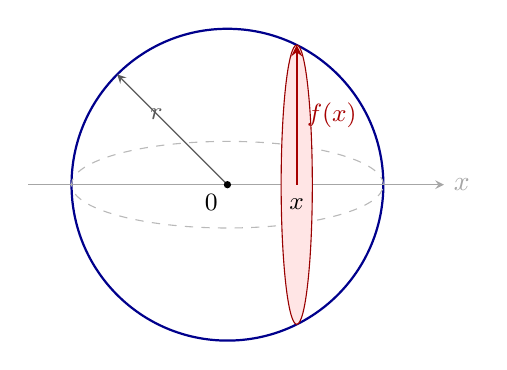
\begin{tikzpicture}[scale=1.1,>=stealth]
  \draw[blue!55!black,thick] (0,0) circle(1.8);
  \draw[gray!55,dashed] (0,0) ellipse(1.8 and 0.5);
  \draw[->,gray!70](-2.3,0)--(2.5,0) node[right]{$x$};
  \fill[red!10] (0.8,0) ellipse(0.18 and 1.612);
  \draw[red!60!black] (0.8,0) ellipse(0.18 and 1.612);
  \draw[->,red!65!black,thick] (0.8,0)--(0.8,1.612) node[midway,right]{\small$f(x)$};
  \draw[->,gray!70!black] (0,0)--(-1.273,1.273) node[midway,above left]{\small$r$};
  \fill (0,0) circle(1.2pt);
  \node[below] at (0.8,-0.05){\small$x$}; \node[below left] at (0,0){\small$0$};
\end{tikzpicture}\obrpopis{Objem koule jako součet tenkých plátků: rotací půlkružnice $f(x)=\sqrt{r^2-x^2}$ kolem osy~$x$ vznikne koule. Řez kolmý k~ose v~bodě $x$ je kruh o~poloměru $f(x)=\sqrt{r^2-x^2}$, tj.\ s~obsahem $\pi f(x)^2=\pi(r^2-x^2)$; sečteno integrálem na $[-r,r]$ dává $V=\tfrac{4}{3}\pi r^3$.}
\end{center}
\end{priklad}

\begin{poznamka}
Integrand $r^2-x^2$ je \emph{sudý}, takže šlo počítat zkratkou $V=2\pi\int_0^r(r^2-x^2)\,\mathrm{d}x$ (poloviční interval, dvojnásobek) a vyhnout se zápornému kraji. Rozměrová kontrola: výsledek vyšel úměrný $r^3$, což je objem -- koeficient $\tfrac43\pi$ je bezrozměrný.
\end{poznamka}

% ============================================================
\section*{Shrnutí}
\addcontentsline{toc}{section}{Shrnutí}

\begin{poznamka}
\textbf{Klíčové vlastnosti a vzorce (přehled k~SZZ).} Stručný výčet klíčových definic, vět a vzorců okruhu M1.

\smallskip
\emph{Posloupnosti a limity.}
\begin{itemize}
  \item Limita $\lim_{n\to\infty}a_n=a\in\mathbb{R}$: $\forall\varepsilon>0\ \exists n_0\ \forall n>n_0:\ |a_n-a|<\varepsilon$. Vlastní limita $\Rightarrow$ konvergentní; nevlastní ($\pm\infty$) nebo neexistující $\Rightarrow$ divergentní.
  \item Konvergentní $\Rightarrow$ omezená (ne naopak: $(-1)^n$ je omezená, ale divergentní). Důkaz obměnou: pro $\varepsilon=1$ existuje $n_0$, poté $|a_n|\le|L|+1$; konečně mnoho prvních členů pokryje $K=\max\{|a_1|,\dots,|a_{n_0-1}|,|L|+1\}$.
  \item Monotónní posloupnost vždy má limitu (vlastní $\iff$ navíc omezená).
  \item Aritmetika limit: $\lim(a_n\pm b_n)=A\pm B$, $\lim(a_n b_n)=AB$, $\lim\tfrac{a_n}{b_n}=\tfrac AB$ --- platí, je-li pravá strana definovaná (neurčité výrazy $\infty-\infty$, $0\cdot\infty$ vyloučeny). Omezená $\cdot$ nulová $= 0$.
  \item Věta o~dvou policajtech: $a_n\le c_n\le b_n$ a $\lim a_n=\lim b_n=L$ $\Rightarrow$ $\lim c_n=L$.
  \item Limita a uspořádání: z $A<B$ plyne $a_n<b_n$ od jistého indexu; z $a_n\le b_n$ pro vš.\ $n$ plyne $A\le B$ (ostrá nerovnost se v limitě může zkazit na neostrou).
\end{itemize}

\smallskip
\emph{Řady.}
\begin{itemize}
  \item Řada $\sum_{n=0}^\infty a_n$: $N$-tý částečný součet $s_N=\sum_{n=0}^N a_n$; konverguje $\iff\lim_{N\to\infty}s_N\in\mathbb{R}$.
  \item Nutná podmínka konvergence: $a_n\to0$. Nestačí --- harmonická $\sum_{n\ge1}\tfrac1n$ diverguje, přestože $\tfrac1n\to0$.
  \item Geometrická řada $\sum_{n\ge0}q^n$: pro $|q|<1$ součet $\tfrac{1}{1-q}$; pro $q\ge1$ součet $+\infty$; pro $q\le-1$ součet neexistuje. Mezivýsledek: $s_N=\tfrac{q^{N+1}-1}{q-1}$ pro $q\neq1$.
  \item $p$-série $\sum_{n\ge1}\tfrac{1}{n^s}$: konverguje pro $s>1$, diverguje pro $s\le1$ (integrálním kritériem).
\end{itemize}

\smallskip
\emph{Limita funkce a spojitost.}
\begin{itemize}
  \item $\lim_{x\to a}f(x)=A$: $\forall\varepsilon>0\ \exists\delta>0:\ x\in P(a,\delta)\Rightarrow|f(x)-A|<\varepsilon$. Limita oboustranná $\iff$ obě jednostranné existují a rovnají se; totéž pro $a,A\in\mathbb{R}^*$ přes okolí $\pm\infty$.
  \item Heineho věta: $\lim_{x\to a}f(x)=A$ $\iff$ pro každou $x_n\to a$, $x_n\neq a$, platí $f(x_n)\to A$. Hodí se k důkazu neexistence limity (stačí najít dvě posloupnosti s různými limitami $f(x_n)$, $f(y_n)$).
  \item Aritmetika limit, limita a uspořádání, věta o dvou policajtech: analogicky jako u posloupností.
  \item Limita složené funkce: $\lim_{x\to a}g=B$, $\lim_{y\to B}f=C$ a navíc (P1) $f$ spojitá v~$B$, nebo (P2) $g$ na okol.\ $a$ nenabývá hodnoty $B$ $\Rightarrow$ $\lim_{x\to a}f(g(x))=C$. (Bez P1/P2 může selhat.)
  \item Spojitost $f$ v~$a$: $\lim_{x\to a}f(x)=f(a)$. Nespojitost: limita neexistuje, nebo existuje, ale $\neq f(a)$. Pokud $f$ v~$a$ není definována, o (ne)spojitosti nelze mluvit.
  \item Darbouxova věta: $f$ spojitá na~$[a,b]$ $\Rightarrow$ nabývá každé hodnoty mezi $f(a)$ a~$f(b)$ (zobrazuje interval na interval). Aplikace: metoda půlení intervalů pro kořeny.
  \item Princip maxima: $f$ spojitá na~kompaktním $[a,b]$ $\Rightarrow$ nabývá svého maxima i~minima. Uzavřenost nutná ($f(x)=x$ na $(0,1)$ max ani min nemá).
\end{itemize}

\smallskip
\emph{Derivace a aplikace.}
\begin{itemize}
  \item Definice: $f'(b)=\lim_{h\to0}\tfrac{f(b+h)-f(b)}{h}$. Diferencovatelnost $\Rightarrow$ spojitost (ne naopak: $|x|$ v~$0$).
  \item Pravidla: $(f+g)'=f'+g'$, $(\alpha f)'=\alpha f'$, $(fg)'=f'g+fg'$ (Leibniz; u nevlastních derivací navíc $f$ nebo $g$ spojitá), $\bigl(\tfrac fg\bigr)'=\tfrac{f'g-fg'}{g^2}$ ($g$ spojitá, $g(b)\neq0$); $(f\circ g)'(a)=f'(g(a))\cdot g'(a)$ (řetízkové); $(f^{-1})'(y_0)=\tfrac{1}{f'(x_0)}$ (inverze, $f'(x_0)\neq0$).
  \item Základní derivace: $(x^n)'=nx^{n-1}$, $(e^x)'=e^x$, $(\ln x)'=\tfrac1x$, $(\sin x)'=\cos x$, $(\cos x)'=-\sin x$, $(\arctan x)'=\tfrac{1}{1+x^2}$.
  \item l'Hospitalovo pravidlo: $\lim\tfrac fg=\lim\tfrac{f'}{g'}$ (pokud pravá strana existuje), platí pro neurčité výrazy $\tfrac00$ a~$\tfrac\infty\infty$. U jiných výrazů \emph{nelze} použít; neexistence limity $f'/g'$ nic neříká.
  \item Nutná podmínka lokálního extrému: $f'(a)=0$ nebo derivace neexistuje (vč.\ krajních bodů). Monotonie: $f'>0\Rightarrow$ rostoucí, $f'<0\Rightarrow$ klesající, $f'\equiv0\Rightarrow$ konstantní.
  \item Konvexita: $f''>0\Rightarrow$ ryze konvexní, $f''<0\Rightarrow$ ryze konkávní; inflexní bod = změna konvexity.
  \item Rolleova věta: $f$ spoj.\ na $[a,b]$, diff.\ na $(a,b)$, $f(a)=f(b)$ $\Rightarrow\exists c\in(a,b):f'(c)=0$. Lagrangeova: totéž bez podmínky $f(a)=f(b)$, $\exists c:f'(c)=\tfrac{f(b)-f(a)}{b-a}$ (tečna rovnoběžná se sečnou krajních bodů).
  \item Taylorův polynom řádu $n$ v~$a$: $T_n^{f,a}(x)=\sum_{i=0}^{n}\tfrac{f^{(i)}(a)}{i!}(x-a)^i$; jediný polynom stupně $\le n$ s~$f(x)-T_n=o(|x-a|^n)$ pro $x\to a$. Lagrangeův zbytek: $\tfrac{f^{(n+1)}(c)}{(n+1)!}(x-a)^{n+1}$ pro nějaké $c$ mezi $a$ a~$x$.
  \item Maclaurinovy rozvoje ($a=0$): $e^x=\sum_{n\ge0}\tfrac{x^n}{n!}$, $\sin x=x-\tfrac{x^3}{3!}+\tfrac{x^5}{5!}-\cdots$, $\cos x=1-\tfrac{x^2}{2!}+\tfrac{x^4}{4!}-\cdots$, $\ln(1+x)=x-\tfrac{x^2}{2}+\tfrac{x^3}{3}-\cdots$
\end{itemize}

\smallskip
\emph{Integrály a aplikace.}
\begin{itemize}
  \item Primitivní funkce $F$ k~$f$ na~$I$: $F'(x)=f(x)$ pro vš.\ $x\in I$. Dvě primitivní funkce k~téže $f$ na intervalu se liší o~konstantu; každá spojitá funkce primitivní funkci má.
  \item Substituce: $\int f(\varphi(t))\,\varphi'(t)\,\mathrm{d}t=F(\varphi(t))+c$ (řetízkové pravidlo pozpátku). U~určitého integrálu přepočítat meze: $\int_{t_1}^{t_2}f(\varphi(t))\,\varphi'(t)\,\mathrm{d}t=\int_{\varphi(t_1)}^{\varphi(t_2)}f(x)\,\mathrm{d}x$.
  \item Per partes: $\int f(x)G(x)\,\mathrm{d}x=F(x)G(x)-\int F(x)g(x)\,\mathrm{d}x$ (Leibnizovo pravidlo pozpátku). Typické výsledky: $\int x\sin x\,\mathrm{d}x=\sin x-x\cos x+c$, $\int x\cos x\,\mathrm{d}x=\cos x+x\sin x+c$.
  \item Newtonův integrál: $(N)\!\int_a^b f=[F]_a^b=F(b)-F(a)$ (nezávisí na volbě~$F$).
  \item Riemannův integrál: $\sup$ dolních sum $=$ $\inf$ horních sum (a obě konečné) $\Rightarrow$ $f$ integrovatelná. Postačující podmínka: $f$ spojitá nebo $f$ monotónní na $[a,b]$.
  \item 1.~základní věta analýzy: $F(x)=\int_a^x f(t)\,\mathrm{d}t\Rightarrow F'(x_0)=f(x_0)$ v~bodech spojitosti $f$. 2.~základní věta: pro $f\in R[a,b]\cap N(a,b)$ je Riemannův $=$ Newtonův (pro spojité $f$ vždy).
  \item Obsah: plocha pod grafem $f\ge0$ na $[a,b]$ je $\int_a^b f(x)\,\mathrm{d}x$.
  \item Odhad sumy integrálem: $f$ nerostoucí $\Rightarrow\sum_{k=1}^{n-1}f(k)\ge\int_1^n f\ge\sum_{k=2}^{n}f(k)$ (pro neklesající $f$ nerovnosti opačně). Integrální kritérium: $f\ge0$ nerostoucí $\Rightarrow\sum_{k\ge1}f(k)$ konverguje $\iff\int_1^\infty f<\infty$.
  \item Rotační těleso (rotace $f\ge0$ na $[a,b]$ kolem osy~$x$): objem $V=\pi\int_a^b f(t)^2\,\mathrm{d}t$, povrch $S=2\pi\int_a^b f(t)\sqrt{1+(f'(t))^2}\,\mathrm{d}t$.
  \item Délka křivky (grafu $f$): $L=\int_a^b\sqrt{1+(f'(t))^2}\,\mathrm{d}t$.
\end{itemize}
\end{poznamka}

% ============================================================
\section*{Zdroje}
\addcontentsline{toc}{section}{Zdroje}

{\raggedright
\begin{itemize}
  \item V.~Jelínek: \emph{Matematická analýza 1}, kompletní zápisky z~přednášky NMAI054, MFF UK, 2019/20 (primární zdroj výkladu).\\ \url{https://iuuk.mff.cuni.cz/~jelinek/1920/ma1.html}
  \item L.~Pick, S.~Hencl, J.~Spurný, M.~Zelený: \emph{Matematická analýza}, skripta (verze 2025-02-09).\\ \url{https://www.karlin.mff.cuni.cz/~pick/analyza-pro-studenty-2025-02-09.pdf}
  \item L.~Pick: \emph{Sbírka příkladů k~MA I a II}.\\ \url{https://www.karlin.mff.cuni.cz/~pick/sbirka.pdf}
  \item 3Blue1Brown: \emph{Essence of Calculus} (videa odkazovaná v~textu).\\ \url{\playlist}
  \item MFF UK: požadavky ke státní závěrečné zkoušce (Informatika, Bc.) a zadání otázek z~minulých termínů.\\ \url{https://www.mff.cuni.cz/cs/studenti/bakalarske-studium/statni-zaverecne-zkousky/bakalarske-statni-zkousky-studijniho-programu-informatika}
\end{itemize}
\par}

\end{document}
